\documentclass[conference]{IEEEtran}
\IEEEoverridecommandlockouts
\usepackage{cite}
\usepackage{amsmath}
\usepackage{newtxtext,newtxmath}   % Times-compatible text+math (matches IEEE template)
\usepackage{graphicx}
\usepackage{booktabs}
\usepackage{url}
\usepackage{xcolor}
\usepackage[hidelinks]{hyperref}

\begin{document}

% --- Camera-ready copyright notice ---
% IEMCON provides the exact string (with the proceedings ISBN) via IEEE eCopyright/EDAS,
% and many IEEE conferences stamp it automatically -- check the IEMCON 2026 camera-ready
% instructions. If you must embed it, uncomment and fill in the ISBN below (place BEFORE
% \maketitle):
% \IEEEpubid{\makebox[\textwidth]{979-8-XXXX-XXXX-X/26/\$31.00~\copyright{}2026 IEEE\hfill}}

\title{Reachability Is Not Consequence:\\
Consequence-Aware Prioritization of Identity Risk\\
in Cloud-Native Infrastructure\\
\thanks{Aspects of this work are the subject of pending U.S.\ patent applications
(No.~19/641,446 and No.~64/138,302).}}

\author{\IEEEauthorblockN{Prawal Pokharel}
\IEEEauthorblockA{\textit{Iverson Cloud} \\
Euless, TX, USA \\
prawal.pokharel7@gmail.com}}

\maketitle

\begin{abstract}
Identity and access management (IAM) has become the dominant attack surface of
cloud-native infrastructure, and the standard defensive posture---least privilege
by access analysis---ranks identities by what they can reach: how many permissions
they hold, whether those permissions are privileged, how many resources they can
touch. We show that this reachability view systematically misranks identity risk,
because it is blind to what fails downstream when reached resources are abused. An
identity holding a single write capability on a shared cache that half the cluster
depends on is more dangerous than one holding administrative rights on a leaf
service that nothing depends on, yet every access-based metric scores them
identically or inverts them. We formalize \emph{identity blast radius}: the
consequence of compromising an identity, obtained by joining the authorization
graph to the runtime service-dependency graph and propagating consequence through
it along three channels---availability, confidentiality, and integrity. Against
ground truth computed by a production dependency-analysis engine over five real
infrastructure topologies, identity blast radius achieves rank correlation
$\rho=0.67$--$0.74$ with true consequence, while the strongest reachability
baseline reaches only $0.29$--$0.44$. We then close the paper's central
methodological gap with \emph{real} experiments on a live Kubernetes cluster: under
scale-to-zero fault injection on Google's Online Boutique, the consequence-aware
prediction tracks \emph{observed} per-service outages at $\rho=0.987$ (versus
$0.778$ for a naive static graph) and predicted identity blast radius tracks that
observed consequence at $\rho=0.958$; and under \emph{real compromise} experiments with
live RBAC, predicted confidentiality and integrity blast radii reproduce the verified
exfiltration and tampering reach, catching over-privilege that dependency-only views
($\rho=0.69$, $0.26$) miss, while a read-only agent identity neither reads nor tampers.
The availability findings also reproduce on an application outside the model's
development distribution. Because ground truth in these experiments is observed system
behavior rather than the engine's own computation, they remove the computed-oracle
circularity for availability and ground the confidentiality and integrity channels in
real compromise. The effect is
actionable---consequence-guided revocation removes $1.5$--$1.7\times$ more risk per
action than privilege-count guidance---and scales to $10^5$ identities in seconds.
\end{abstract}

\begin{IEEEkeywords}
identity and access management (IAM), cloud-native security, blast radius,
attack-path analysis, privilege escalation, risk prioritization, fault injection,
Kubernetes
\end{IEEEkeywords}

\section{Introduction}
The security center of gravity in cloud infrastructure has moved from the network
perimeter to identity. As workloads decompose into hundreds of services, each
authenticating to others and to managed cloud resources, the number of
identities---human operators, service accounts, workload identities, machine
principals---grows faster than any team can audit, and over-permissioned identities
are pervasive: a recent measurement study of real serverless applications found
that $47.7\%$ carry excess permissions and $18.8\%$ hold unnecessary
privilege-escalation capabilities~\cite{overpriv}. The defensive response is
near-universal: enforce least privilege, and to find where least privilege is
violated, analyze access. Tools that map identity-to-resource reachability---cloud
provider access analyzers, permission-mapping utilities~\cite{awsiam}, Kubernetes
RBAC scanners~\cite{kubiscan}, and the attack-path analyzers descended from
graph-based enumeration~\cite{heatray,bloodhound}---answer the question \emph{what
can this identity reach?} and rank identities by the breadth or privilege of that
reach.

We argue this question is the wrong one. Reachability measures the access an
identity holds, not the consequence of that access being abused. Consider two
identities: one holds a single write capability on a shared cache a dozen services
read on every request, so compromising it degrades the checkout path and the
user-facing storefront through the dependency graph; the other holds full
administrative control over a nightly batch job nothing depends on, so compromising
it degrades exactly one workload. Every reachability metric---permission count,
privileged-role count, reachable-resource count---ranks the second at least as
dangerous as the first, because it holds more, and more privileged, access. The
dependency structure says the opposite: the danger of an identity is not what it
can touch but what fails when what it can touch is abused---a property of the
infrastructure it sits above, not of its permission list.

This paper makes that intuition precise and measures it. We formalize identity
blast radius as the join of two graphs the field already builds separately: the
authorization graph, which says which identities can affect which resources, and
the runtime service-dependency graph, which says what happens when a resource is
abused. Ranking identities by the propagated consequence of the access they hold,
rather than by the access itself, is our contribution. Our evidence comes in three
tiers of increasing realism. Against \emph{exact synthetic} consequence and the
output of a \emph{production dependency-analysis engine} (Iverson Cloud) over five
real topologies, consequence-aware ranking is substantially more faithful to true
risk than any access-based ranking, and the two rankings disagree on the identities
that matter most. We then add a third tier that answers the sharpest objection to
oracle-based evaluation---that the oracle and the estimator might share
structure---by validating predicted blast radius against \emph{observed} system
behavior: real scale-to-zero fault injection on a live microservice cluster
(availability) and real read/write compromise with live Kubernetes RBAC
(confidentiality and integrity). Ground truth is measured, not computed, and the
consequence-aware prediction tracks it.

\section{Related Work}
\textbf{Identity and access analysis.} A large body of tooling analyzes cloud and
cluster authorization to surface excessive privilege. Cloud-provider access
analyzers and permission-mapping tools enumerate the resources a principal can
reach and flag broad or unused grants, and generate least-privilege policies from
logged activity~\cite{awsiam}; static overprivilege analysis of cloud policies
detects excessive permissions in serverless applications by reasoning about which
resources a function may touch~\cite{overpriv}. Kubernetes-specific scanners
enumerate RBAC bindings and highlight wildcard, cluster-admin, and secret-reading
permissions~\cite{kubiscan}. Graph-based attack-path analysis, in the lineage of
the identity-snowball model of Heat-ray~\cite{heatray} and popularized by
BloodHound~\cite{bloodhound}, computes reachability paths from a principal to a
high-value target and has driven substantial follow-on work on hardening such
graphs by edge blocking~\cite{gecco}. The cloud analogue models authorization
policies themselves as reachability graphs: Grasp, for instance, renders serverless
IAM policies as queryable reachability graphs to find which principals can reach
which resources~\cite{grasp}. All of these answer a reachability question---which
resources, how privileged, how many hops---and rank findings by properties of the
access itself. None incorporates the downstream infrastructure consequence of
abusing that access, which is the axis this paper adds.

\textbf{Dependency and blast-radius analysis.} A separate line of work models
service dependency graphs for reliability: identifying critical services,
predicting cascading failure, and quantifying the blast radius of a workload's
degradation~\cite{aid,failsurvey}. This literature explicitly argues that
reliability engineers should prioritize services with greater downstream
impact~\cite{aid} and surveys cascading-failure diagnosis in microservice
systems~\cite{failsurvey}, but applies the idea to fault tolerance, not to identity
risk. Our contribution is to use a dependency/blast-radius engine as the
consequence oracle for identities, by composing per-workload blast radius through
the authorization graph.

\textbf{Least privilege and RBAC mining.} Role-based access control~\cite{rbac,nist}
is the dominant authorization model in the settings we study, and a long line of
role-mining and policy-rightsizing methods infers minimal roles from existing
assignments and observed usage~\cite{rmp,roleminer,rminesurvey,semrole}, typically
treating a permission as removable if it is unused over an observation
window~\cite{awsiam}. Most of this work weights permissions uniformly or by usage
frequency; the observation that permissions differ in intrinsic severity has been
raised~\cite{severity} but not connected to downstream infrastructure consequence.
This usage view is orthogonal and complementary to ours: it asks whether a
permission is needed, while we ask what a permission endangers. We return to the
interaction between usage evidence and consequence in the discussion.

To our knowledge, no prior system ranks identities by the propagated infrastructure
consequence of the access they hold, nor demonstrates that access-based ranking and
consequence-based ranking disagree on the identities that matter most.

\section{Problem Formulation}
\subsection{The joined graph}
An infrastructure estate comprises a set of resources (workloads, data stores,
managed services) $V$ and a directed dependency relation $D \subseteq V \times V$,
where $(a,b) \in D$ means ``$a$ depends on $b$'': if $b$ degrades, $a$ is impaired.
For $r \in V$, write $\Delta(r)$ for its transitive \emph{dependents} (ancestors
under $D$---what fails if $r$ fails) and $\nabla(r)$ for its transitive
\emph{dependencies} (descendants under $D$---what $r$ draws upon). The estate also
hosts a set of identities $I$. Authorization is a labeled relation $A \subseteq I
\times V \times C$, where $(i,r,c) \in A$ means identity $i$ holds capability $c$ on
resource $r$, and $C$ is an ordered set of capability classes (Table~\ref{tab:caps}).

\subsection{Availability blast radius}
For a resource $r$, degrading $r$ impairs every member of $\Delta(r)$. We attach to
each resource a consequence weight; in the deployments studied here the consequence
of losing a resource is measured by a production dependency engine as the size and
user-facing reach of its downstream set (Section~\ref{sec:setup}). Writing
$\mathrm{bl}(r)$ for that engine-measured blast radius, the identity blast radius of
$i$ aggregates, over every resource $i$ can destroy, the severity of the capability
and the consequence of degrading that resource:
\begin{equation}
\mathrm{IBR}_A(i) = \!\!\!\sum_{\substack{(i,r,c)\in A\\ c\ \text{destructive}}}\!\!\!
 w(c)\,\bigl(\kappa(r) + \lambda\,\mathrm{bl}(r)\bigr),
\label{eq:ibr}
\end{equation}
where $\kappa(r)$ is the resource's own criticality and $\lambda$ scales the
downstream term. The ground-truth availability consequence of compromising $i$ is
the actual set of resources that fail when $i$ exercises all of its destructive
capabilities---the union of downstream sets of the resources $i$ can
degrade---weighted by user-facing reach.

\subsection{Confidentiality and integrity channels}
\label{sec:ci}
Availability is only one axis of consequence. A capability that reads a resource
does not degrade it, so it contributes nothing to Eq.~\eqref{eq:ibr}, yet a read on
a resource that aggregates sensitive data---or that holds credentials to its own
dependencies---can have large confidentiality consequence. We therefore extend the
same joined graph with two further channels, propagating in the directions dictated
by the semantics of each channel.

\emph{Confidentiality} flows \emph{down} the dependency graph: reading a resource
$r$ exposes $r$'s own data and, transitively, the data of everything $r$ draws
upon, because a compromised service yields the credentials it uses to reach its
dependencies. With read potency $\rho(c)$ (how much a read-class capability
exposes; $\mathrm{SECRET\_READ}$ far exceeds metadata reads) and per-store
sensitivity $\sigma(s)$,
\begin{equation}
\mathrm{IBR}_C(i) = \!\!\!\sum_{\substack{(i,r,c)\in A\\ c\ \text{read-like}}}\!\!\!
 \rho(c)\!\!\sum_{s\,\in\,\{r\}\cup\nabla(r)}\!\!\!\sigma(s).
\label{eq:conf}
\end{equation}
\emph{Integrity} flows \emph{up}, like availability, but is gated by write potency
$\pi(c)$: corrupting $r$ propagates to the dependents $\Delta(r)$ that trust $r$'s
data. The combined consequence is the normalized sum of the three channels. This
extension is what lets the framework score a pure secret-reader---invisible to
Eq.~\eqref{eq:ibr}---and is validated both on synthetic ground truth and against
real exfiltration (Section~\ref{sec:ci-results}).

\subsection{Reachability baselines as degenerate cases}
Setting the downstream term to zero ($\lambda=0$, $\kappa$ constant) reduces
Eq.~\eqref{eq:ibr} to a count of destructive permissions weighted by
capability---an access-only score. Dropping the capability weight as well yields a
pure reachable-resource count. The baselines we compare against are exactly these
degeneracies, plus common variants: \textbf{PermCount} (permissions held),
\textbf{PrivRoleCount} (privileged capabilities held), \textbf{ReachCount} (distinct
resources reachable), \textbf{ReachCrit} (reachable resources weighted by static
criticality---the strongest reachability baseline), \textbf{IBR-noDep}
(Eq.~\eqref{eq:ibr} with $\lambda=0$), and \textbf{IBR-full}.

\begin{table}[t]
\caption{Capability classes and severity weights. Only the \emph{ordering} affects
availability results (Section~\ref{sec:scale}); destructive classes can degrade a
resource.}
\label{tab:caps}
\centering
\begin{tabular}{lcc}
\toprule
Capability class & Weight $w(c)$ & Destructive \\
\midrule
READ & 0.20 & no \\
WRITE & 0.50 & yes \\
EXECUTE & 0.85 & yes \\
SECRET\_READ & 0.90 & no (availability) \\
ADMIN & 1.00 & yes \\
\bottomrule
\end{tabular}
\end{table}

\section{Experimental Setup}
\label{sec:setup}
We evaluate on three tiers of increasing realism.

\textbf{Tier A: synthetic estates with constructed ground truth.} A seeded generator
emits estates with a parameterized identity population (human, service, and machine
principals), an authorization layer with tunable privilege mix and wildcard
prevalence, and a layered scale-free dependency graph in which preferential
attachment produces a realistic minority of high-in-degree ``single point of
failure'' resources. Because the estate is generated, the true consequence of
compromising any identity is computable directly from the generative model,
independent of any scoring method. Identity counts are swept from $10^2$ to $10^5$.

\textbf{Tier B: real topologies with a production consequence oracle.} We drive the
Iverson Cloud dependency-analysis engine over five real infrastructure topologies
shipped as its evaluation fixtures: a cloud microservice estate, a GPU-training
cluster, a drone-swarm control network, an underwater acoustic-positioning network,
and a strategic-communications topology. For the worked examples we additionally use
Google's Online Boutique, whose service call graph is publicly documented~\cite{ob}.
For each topology the engine computes, per workload, the directed
confidence-weighted blast radius. We then synthesize identity populations over the
real workloads and take the ground-truth consequence of an identity to be the union
of the engine's blast radii for the workloads it can destroy.

\textbf{Tier C: live-cluster fault injection and real compromise.} The prior tiers
take consequence from an engine's computation, which invites the objection that
estimator and oracle share dependency structure. Tier C removes that objection by
measuring \emph{observed} consequence on a live cluster. We deploy the real Online
Boutique (eleven microservices) on Kubernetes and, for the availability channel,
inject faults by scaling each service to zero and recording which real user-facing
flows break over HTTP; for the confidentiality and integrity channels, we stand up
real Kubernetes Secrets, ConfigMaps, ServiceAccounts, and RBAC and ``compromise'' each
identity by actually reading the secrets, and corrupting the data-of-record, its
credentials reach---chaining laterally. Ground truth in Tier~C is measured system
behavior, not any computation of ours. Before an identity's kill/compromise we confirm
the target is truly removed and the baseline is healthy, isolating each measurement. To
test generalization beyond the app the dependency heuristic was developed on, we repeat
the availability fault injection on Istio's Bookinfo (Section~\ref{sec:offdist}).

\textbf{Protocol and metrics.} Every experiment scores each identity with the full
battery and compares each method's induced ranking to the ground-truth ranking. We
report Spearman $\rho$ over the full ranking and set overlap for the top-$k$
identities, since the operational task is top-heavy. All experiments regenerate from
fixed seeds; generator, synthesizer, scoring battery, and figure scripts are
released.\footnote{Reproducibility repository: \texttt{github.com/prawalpokharel/CEI-Cloud-Identity-IEEE}.}

\section{Results}
\subsection{Access-based ranking is systematically wrong (synthetic)}
Over 40 seeded estates of 500 identities each, Fig.~\ref{fig:synth} reports rank
correlation with true consequence. The reachability baselines correlate
weakly---PrivRoleCount $\rho=0.41$, PermCount and ReachCount $0.57$, and even
criticality-weighted ReachCrit only $0.67$---while the full method reaches
$\rho=0.93$. The ablation is visible here: removing the dependency join (IBR-noDep)
drops correlation to $0.81$, and the gap between ReachCrit and IBR-full is precisely
the value of joining the dependency graph. The top-$k$ most-critical identities
under ReachCrit and IBR-full overlap by only about half (Jaccard $\approx0.49$--
$0.51$ for $k\in\{5,10,25\}$): an analyst working a reachability-ranked queue would
spend roughly half their effort on the wrong identities.

\begin{figure}[t]
\centering
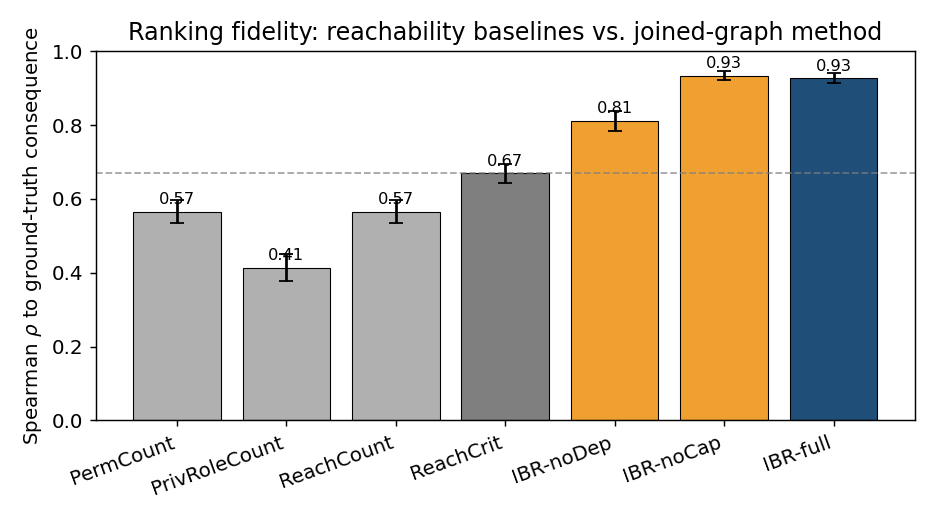
\includegraphics[width=\columnwidth]{figures/fig_e2_ranking.png}
\caption{Ranking fidelity to constructed ground truth (40 estates, 500 identities
each). Reachability baselines (grey) correlate weakly; the dependency join (blue)
closes the gap. Error bars are standard deviation across estates.}
\label{fig:synth}
\end{figure}

\subsection{The same result against a production engine on real topologies}
The synthetic result could be an artifact of the generative model. We repeat the
comparison with ground truth supplied by the real engine over Online Boutique.
Fig.~\ref{fig:engine} shows the same ordering, more sharply: the resource-counting
baselines collapse to $\rho=0.31$---ReachCrit included, because the engine assigns
no separating static criticality on this topology---while IBR-full reaches
$\rho=0.71$ and IBR-noDep sits between at $0.51$. The engine reports that
\texttt{redis-cart} degrades three downstream services including the user-facing
frontend, while a synthesized nightly-reconciler batch job degrades nothing; a
single write capability on the former outranks administrative capability on the
latter, and no reachability metric can express the difference.

\begin{figure}[t]
\centering
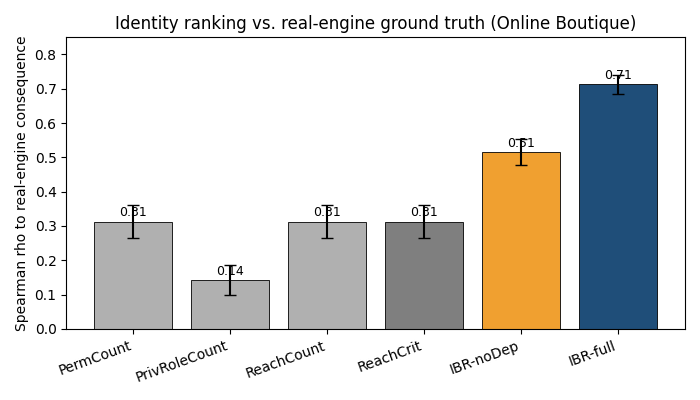
\includegraphics[width=\columnwidth]{figures/fig_e8_real_engine.png}
\caption{Ranking fidelity against ground truth from the production engine over
Online Boutique (30 populations, 400 identities each). The resource-counting baselines
collapse to $\rho=0.31$ (privileged-role counting lower still, $0.14$); the dependency
join reaches $0.71$.}
\label{fig:engine}
\end{figure}

\subsection{Why: the dependency join and the low-privilege danger}
The strongest predictor of reachability under-ranking is the maximum downstream
fan-out of the resources an identity can reach: identities whose few permissions
land upstream of large dependency cascades are exactly the ones reachability misses.
Fig.~\ref{fig:depth} makes the mechanism visible: as fan-out depth grows, the
reachability baseline's recall of the top-10 riskiest identities degrades from
$0.40$ to $0.16$, while the dependency-aware method stays substantially higher. The
practical face of this mechanism is the low-privilege, high-consequence
identity---few permissions, no privileged role, yet atop a large blast
radius---invisible to privilege-focused review.

\begin{figure}[t]
\centering
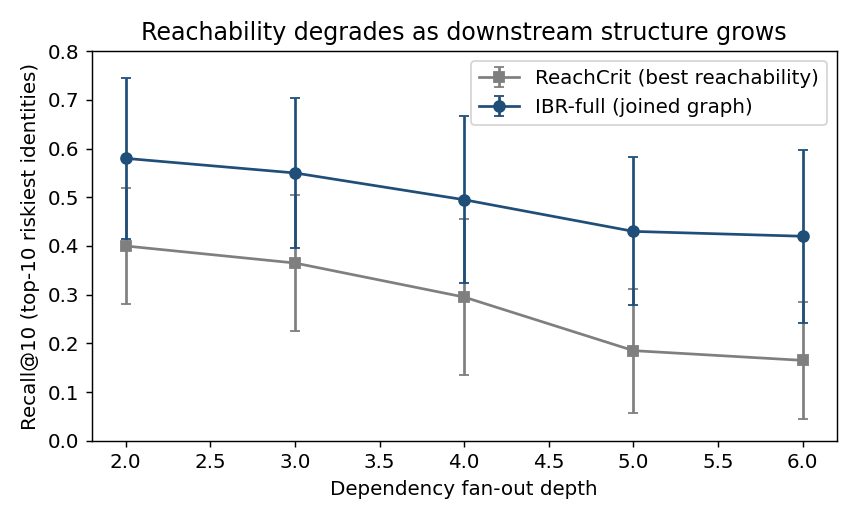
\includegraphics[width=\columnwidth]{figures/fig_e3_recall_vs_depth.png}
\caption{Recall@10 of the riskiest identities versus dependency fan-out depth.
Reachability degrades as there is more downstream structure to ignore.}
\label{fig:depth}
\end{figure}

\subsection{The result generalizes across real topologies}
Fig.~\ref{fig:cross} repeats the real-engine comparison across all five shipped
topologies. The gap holds everywhere: mean rank correlation rises from $0.38$ for
reachability to $0.72$ for the dependency-aware method, and---consistent with the
mechanism---the gap is widest on the topologies whose maximum blast radius is
deepest (the drone-swarm and GPU-cluster estates, with engine-measured blast radii
up to $11$--$12$ downstream workloads).

\begin{figure}[t]
\centering
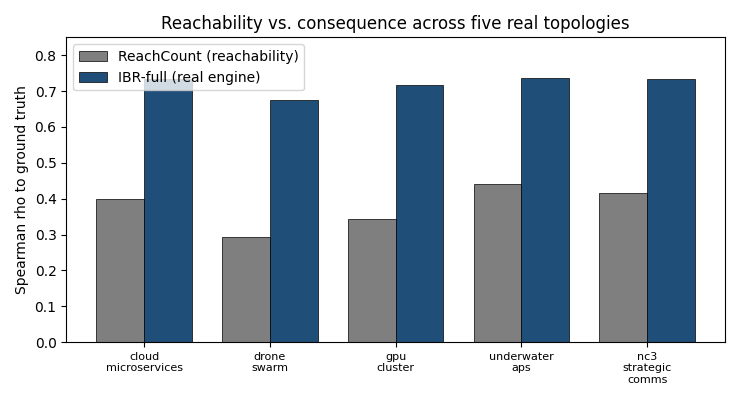
\includegraphics[width=\columnwidth]{figures/fig_e9_cross_topology.png}
\caption{Rank correlation with real-engine ground truth across five real topologies.
The reachability-to-consequence gap is present in every case (mean $0.38\to0.72$).}
\label{fig:cross}
\end{figure}

\subsection{Real fault injection: predicted blast radius vs.\ observed outages}
\label{sec:real-avail}
Tiers A and B take consequence from a computation. We now measure it. On the live
Online Boutique cluster we scale each backend service to zero---a real, reversible
fault---and record which of five real user-facing flows (home, browse, add-to-cart,
view-cart, checkout) actually break over HTTP. The ground truth is the
\emph{observed} outage, independent of the engine's graph.

Fig.~\ref{fig:tierc} reports the result. Three services---the ad, email, and
recommendation services---break \emph{no} user-facing flow when removed: the
frontend degrades gracefully. A naive static graph, which treats every declared
dependency edge as failure-propagating, over-predicts exactly these three; the
confidence-aware prediction, which the engine already computes, matches the observed
broken-flow set on $8$ of $10$ services and reaches Spearman $\rho=0.987$ against
measured blast radius, versus $0.778$ for the naive static graph. Lifting the
measurement to identities---scoring synthesized identities against the
\emph{observed} per-service consequence---predicted identity blast radius tracks
measured consequence at $\rho=0.958$. The two services the confidence-aware model
still over-predicts (currency, product-catalog) are under-broken because the
frontend \emph{caches} their data---a stateful runtime effect no static graph
captures, and a concrete instance of the dynamic-behavior gap we discuss in
Section~\ref{sec:disc}. Crucially, because ground truth here is observed HTTP
failure rather than the engine's own computation, estimator and oracle no longer
share a computed \emph{output}---though both still derive connectivity from the same
deployment manifests, so the independence is behavioral, not structural
(Section~\ref{sec:disc}). This removes the computed-oracle circularity for the
availability channel.

\begin{figure}[t]
\centering
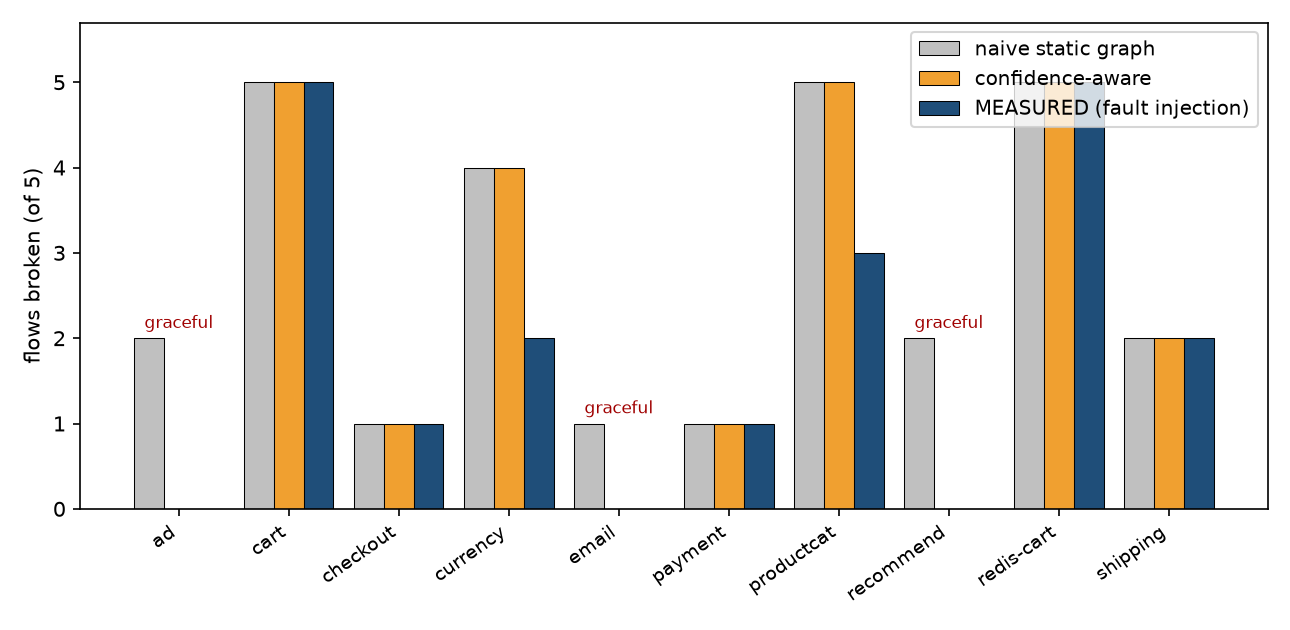
\includegraphics[width=\columnwidth]{figures/fig_tierc_real.png}
\caption{Real fault injection on the live Online Boutique (availability channel). The
naive static graph over-predicts on the three gracefully-degrading services
(ad/email/recommendation); the confidence-aware prediction matches observed reality
($\rho=0.987$).}
\label{fig:tierc}
\end{figure}

\subsection{Confidentiality and integrity, measured under real compromise}
\label{sec:ci-results}
\label{sec:real-conf}
We validate the confidentiality channel (Eq.~\eqref{eq:conf}) twice. First, on
synthetic estates where a confidentiality ground truth is constructible: the
availability-only score of Eq.~\eqref{eq:ibr} correlates with confidentiality
consequence at only $\rho=0.30$, because a pure reader scores near zero; the
three-channel score raises this to $\rho=0.80$, and against a combined
availability$+$confidentiality$+$integrity ground truth the score improves from
$0.83$ to $0.94$. Confidentiality consequence is a distinct axis the
availability-only model does not capture.

Second, and more sharply, we measure real exfiltration. On the live cluster we
create one Secret per service (tagged with a data sensitivity), one ServiceAccount
per service, and RBAC in which a service may read the credential secrets of the
services it calls---plus three realistic over-privilege misconfigurations (an ad
service granted payment credentials, an email service granted the cart store, a
recommendation service granted the cart). We then compromise each identity by
\emph{actually reading} the secrets its RBAC reaches, via live
\texttt{auth can-i}/\texttt{get secret} against the API server, chaining laterally
through each credential recovered. The measured exfiltrated set is the ground truth.
Fig.~\ref{fig:conf} contrasts it with a dependency-only prediction: the
dependency-only view scores $\rho=0.691$ because it cannot see the
misconfigurations, under-rating exactly the over-privileged identities; a
permission-count baseline reaches $0.944$ but ignores the sensitivity-weighted depth
of what is exposed. The confidentiality score computed from the \emph{real extracted
RBAC} reproduces the exfiltrated set ($\rho=1.00$)---not as predictive magic, but
because joining the real authorization graph with the dependency graph recovers the
reach an attacker actually walks; the informative quantity is the gap from $0.69$,
which is precisely the value of extracting real RBAC. Finally, a read-only collector
identity restricted to \texttt{get/list/watch} on pods and services---the posture of
a production topology agent---exfiltrates \emph{zero} secrets under real compromise,
a checkable safety property.

\emph{Integrity} is the dual. We create a ConfigMap data-of-record per service, grant
real \texttt{update} RBAC on the data each service legitimately writes---plus three
over-privilege \emph{write} misconfigurations (ad able to rewrite the product catalog,
email the exchange rates, recommendation the cart)---and compromise each identity by
\emph{actually corrupting} (\texttt{patch -{}-as}) every ConfigMap its RBAC permits,
reading each store back to confirm the tamper. What we observe is the verified
unauthorized \emph{tampering reach}---exactly which data-of-record each identity can
corrupt; the downstream endangered set is attributed through the dependency graph, not by
instrumenting each dependent consuming the bad data, so this is tampering reach with
graph-attributed downstream rather than a fully observed integrity outcome (unlike the
availability channel; Section~\ref{sec:disc}). Against that reach the dependency-only
prediction, blind to the write misconfigurations that hand a low-value identity a
high-fan-out store, collapses to $\rho=0.259$; the RBAC-aware score recovers it
($\rho=1.00$), and the read-only agent corrupts \emph{zero} stores. In both channels the
dependency-only view misses exactly the planted misconfigurations, and extracting the
real authorization graph is what recovers them (Fig.~\ref{fig:conf}).

\begin{figure*}[t]
\centering
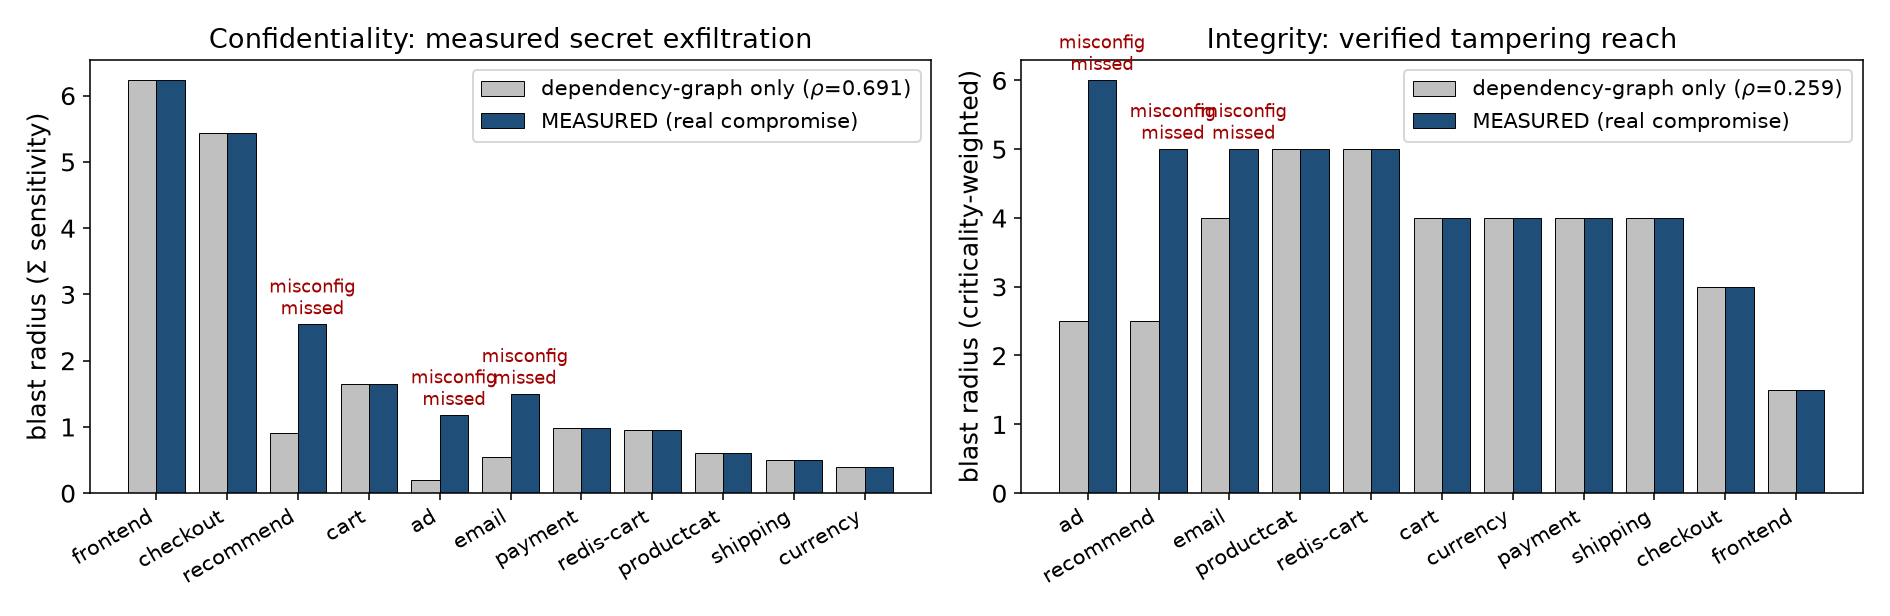
\includegraphics[width=\textwidth]{figures/fig_ci_integrity.png}
\caption{Real credential-compromise (left, confidentiality: measured secret
exfiltration via live reads) and data-tampering (right, integrity: verified tampering
reach via live writes) on the cluster, each versus a dependency-only prediction. The
dependency-only view misses the planted over-privilege misconfigurations (red labels);
the RBAC-aware score recovers the reach in both channels.}
\label{fig:conf}
\end{figure*}

\subsection{Off-distribution validation}
\label{sec:offdist}
A residual concern is that the dependency heuristic was developed on Online Boutique,
so an observed match there is not by itself evidence of generalization. We therefore
repeat the availability fault injection on Istio's Bookinfo---an application the
heuristic was never tuned on, with a different topology (a productpage aggregating a
details service and a reviews service, itself backed by ratings). Under real
scale-to-zero fault injection the user-facing page renders (HTTP~200) when either
backend is removed, degrading only the corresponding section, and goes down only when
the productpage itself is removed. The confidence-aware prediction---that only the
frontend's own failure breaks the page---matches all three observed cases, while the
naive static graph over-predicts, flagging the two gracefully-degrading backends as
page-breaking. The graceful-degradation phenomenon, and the confidence-aware model's
advantage over the static graph, thus reproduce on an application outside the
heuristic's development distribution.

\subsection{Where the capability ladder matters}
The capability effects reported here are weight ablations against constructed and
engine-oracle ground truth (Tiers~A--B), \emph{not} the live-cluster measurements of
Sections~\ref{sec:real-avail}--\ref{sec:real-conf}. The original model reports a plain
negative result for \emph{availability}: the capability weight is second-order---
replacing the binary destructive gate with a per-capability magnitude and then
flattening it changes model-consistency rank correlation by only $0.006$, because the
criticality-plus-downstream term dominates. We confirm this and locate where capability
\emph{does} matter. On the synthetic confidentiality estates (Tier~A), flattening read
potency (so metadata reads and secret reads count alike, an order-of-magnitude span in
the separate read-potency function $\rho(c)$ of Eq.~\eqref{eq:conf}, not the $w(c)$ of
Table~\ref{tab:caps}) drops correlation by $0.070$: the capability ladder is first-order
on the confidentiality channel. Capability severity thus matters exactly where intuition
places it---secret reading---rather than universally, which sharpens rather than
overturns the original finding.

\subsection{Remediation, concentration, and scale}
\label{sec:scale}
A better ranking is only useful if it changes action. Given a budget of one
permission revocation per identity, consequence-guided revocation removes
$1.5$--$1.7\times$ more true engine-measured risk than privilege-count-guided
revocation and up to $2.25\times$ more than random, on every one of the five
topologies (Fig.~\ref{fig:remed}). The ranking also yields a compact defensive
target: the top fifth of workloads by blast radius account for $42$--$64\%$ of all
identity risk (Fig.~\ref{fig:conc}), far above the uniform $20\%$. Finally, the full
scoring battery scores $10^5$ identities in a little over a second (empirical growth
exponent near $1.4$, $\approx 0.01$~ms per identity), and the availability ranking
is stable under every order-preserving perturbation of Table~\ref{tab:caps},
degrading only when the capability \emph{ordering} is shuffled---so it rests on an
ordinal, defensible judgment, not on specific constants.

\begin{figure}[t]
\centering
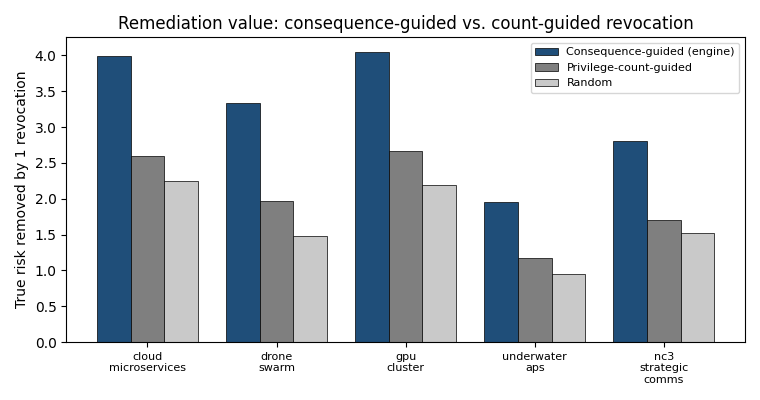
\includegraphics[width=\columnwidth]{figures/fig_e10_remediation.png}
\caption{True risk removed by a single permission revocation, consequence-guided
versus privilege-count versus random, across five topologies.}
\label{fig:remed}
\end{figure}

\begin{figure}[t]
\centering
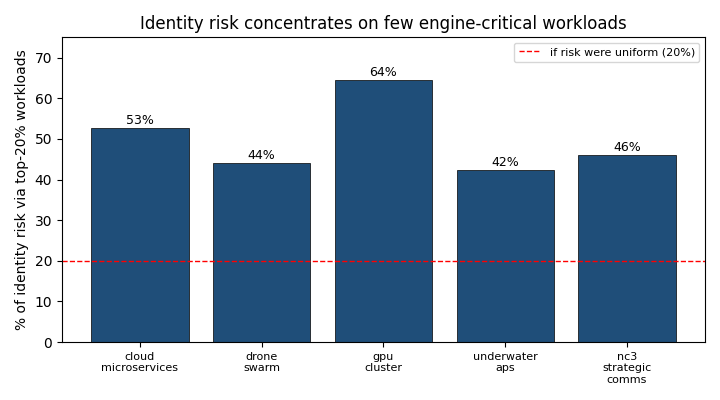
\includegraphics[width=\columnwidth]{figures/fig_e12_concentration.png}
\caption{Share of total identity risk flowing through the top-20\% of workloads by
blast radius. Risk concentrates far above the uniform baseline (dashed).}
\label{fig:conc}
\end{figure}

\section{Discussion and Limitations}
\label{sec:disc}
\textbf{What the evidence shows.} Across three tiers---exact synthetic consequence, a
production engine over five real topologies, and \emph{observed} live-cluster
behavior---consequence-aware ranking is markedly more faithful to true risk than access,
disagrees with it on the identities that matter most, and changes remediation for the
better. The live-cluster experiments are the strongest evidence: they validate predicted
availability blast radius against measured outages, and confidentiality and integrity
against measured exfiltration and data-tampering; because ground truth there is observed
rather than computed, they remove the computed-oracle circularity---decisively for
availability, whose outcome is behaviorally measured rather than computed, and for
confidentiality and integrity up to the shared-RBAC caveat below.

\textbf{Scope of the independence claim.} The fault-injection oracle and the estimator
both derive connectivity from the same deployment manifests, so their independence is
\emph{behavioral}---whether a declared edge actually propagates failure, given graceful
degradation and caching the graph does not encode---not \emph{structural}; the
divergences we report are evidence of that non-identity. To probe generalization we
repeat the injection on Bookinfo (Section~\ref{sec:offdist}), where the same pattern and
advantage hold, though both live studies are small and single-cluster and broader
multi-cluster validation remains future work. The confidentiality and integrity
$\rho=1.00$ reflect that the estimator consumes the same real RBAC the compromise
traverses, so their content is the contrast with the dependency-only $0.69$ and $0.26$,
not the absolute value; the integrity study further verifies which stores each identity
can tamper but attributes downstream corruption through the graph rather than
instrumenting each dependent, so a fully observed integrity oracle remains the natural
next step.

\textbf{Open items.} Usage evidence---whether a high-consequence permission is ever
exercised---is complementary and currently absent: a dormant grant and an actively
used one receive the same score, and the confidentiality result makes this the most
consequential gap, since it now elevates exactly the secret-reading identities for
which ``is it used?'' matters most. Finally, we treat the dependency graph as a
static snapshot; real call graphs shift with traffic, circuit breakers, and feature
flags, and the caching effects in Section~\ref{sec:real-avail} show static fidelity
can decay. Integrating observed-usage and temporal-graph signals with the
consequence signal is the clear extension.

\textbf{Industrial relevance.} Least-privilege programs prioritize by access; this work
shows access and consequence diverge on real infrastructure, and that the information
needed to close the gap---a dependency graph with per-workload blast radius, plus
extracted authorization---is exactly what modern infrastructure-analysis systems already
compute, making consequence ranking deployable on top of dependency analysis clusters
already maintain.

\section{Conclusion}
Identity has become the primary attack surface of cloud infrastructure, and the
standard defense ranks identities by what they can reach. We showed that reachability
systematically misranks identity risk because it ignores dependency structure,
formalized identity blast radius as the join of the authorization and dependency graphs
across availability, confidentiality, and integrity channels, and demonstrated---against
exact synthetic ground truth, a production engine over five real topologies, and
\emph{observed} live-cluster behavior---that consequence-aware ranking is markedly more
faithful to true risk. On real fault injection the prediction tracks observed outages at
$\rho=0.987$ (reproducing off-distribution); on real read and write compromise it recovers
the exfiltrated secrets and verified tampering reach, catching over-privilege that
dependency-only views miss, while a read-only agent identity neither reads nor tampers.
As identity sprawl outpaces human review, prioritizing by propagated consequence rather
than access is both necessary and, atop dependency analysis infrastructure already
performs, practical.

\begin{thebibliography}{00}
\bibitem{heatray} J.~Dunagan, A.~X.~Zheng, and D.~R.~Simon, ``Heat-ray: combating
identity snowball attacks using machine learning, combinatorial optimization and
attack graphs,'' in \emph{Proc. ACM SOSP}, 2009, pp.~305--320.
\bibitem{bloodhound} A.~Robbins, R.~Vazarkar, and W.~Schroeder, ``BloodHound: six
degrees of domain admin,'' presented at DEF CON 24, 2016.
\bibitem{gecco} D.~Goel \emph{et al.}, ``Defending Active Directory by combining
neural network based dynamic program and evolutionary diversity optimisation,'' in
\emph{Proc. GECCO}, 2022, pp.~1191--1199.
\bibitem{overpriv} E.~Yeboah-Duako and P.~Datta, ``Overprivilege analysis of
security policies in serverless cloud applications,'' preprint arXiv:2607.02875,
2026.
\bibitem{grasp} I.~Polinsky, P.~Datta, A.~Bates, and W.~Enck, ``Grasp: hardening
serverless applications through graph reachability analysis of security policies,''
in \emph{Proc. ACM Web Conf. (WWW)}, 2024.
\bibitem{awsiam} Amazon Web Services, ``IAM Access Analyzer policy generation and
least-privilege guidance,'' AWS IAM User Guide, accessed 2026.
\bibitem{kubiscan} CyberArk, ``KubiScan: a tool for scanning Kubernetes clusters for
risky permissions,'' open-source tool, accessed 2026.
\bibitem{rbac} R.~S.~Sandhu, E.~J.~Coyne, H.~L.~Feinstein, and C.~E.~Youman,
``Role-based access control models,'' \emph{IEEE Computer}, vol.~29, no.~2,
pp.~38--47, 1996.
\bibitem{nist} D.~F.~Ferraiolo \emph{et al.}, ``Proposed NIST standard for
role-based access control,'' \emph{ACM TISSEC}, vol.~4, no.~3, pp.~224--274, 2001.
\bibitem{rmp} J.~Vaidya, V.~Atluri, and Q.~Guo, ``The role mining problem: finding a
minimal descriptive set of roles,'' in \emph{Proc. ACM SACMAT}, 2007, pp.~175--184.
\bibitem{roleminer} J.~Vaidya, V.~Atluri, and J.~Warner, ``RoleMiner: mining roles
using subset enumeration,'' in \emph{Proc. ACM CCS}, 2006, pp.~144--153.
\bibitem{rminesurvey} B.~Mitra, S.~Sural, J.~Vaidya, and V.~Atluri, ``A survey of
role mining,'' \emph{ACM Computing Surveys}, vol.~48, no.~4, pp.~1--37, 2016.
\bibitem{semrole} I.~Molloy \emph{et al.}, ``Mining roles with semantic meanings,''
in \emph{Proc. ACM SACMAT}, 2008, pp.~21--30.
\bibitem{severity} S.~V.~Belim, N.~F.~Bogachenko, and A.~N.~Kabanov, ``Severity level
of permissions in role-based access control,'' preprint arXiv:1812.11404, 2018.
\bibitem{aid} T.~Yang \emph{et al.}, ``AID: efficient prediction of aggregated
intensity of dependency in large-scale cloud systems,'' in \emph{Proc. IEEE/ACM
ASE}, 2021, pp.~653--665.
\bibitem{failsurvey} S.~Zhang \emph{et al.}, ``Failure diagnosis in microservice
systems: a comprehensive survey and analysis,'' \emph{ACM TOSEM}, vol.~35, no.~1,
pp.~1--55, 2025.
\bibitem{ob} Google Cloud Platform, ``Online Boutique: a cloud-native microservices
demo application,'' accessed 2026.
\end{thebibliography}

\end{document}
